\documentclass[a4paper, oneside]{book}\usepackage[]{graphicx}\usepackage[]{color}
% maxwidth is the original width if it is less than linewidth
% otherwise use linewidth (to make sure the graphics do not exceed the margin)
\makeatletter
\def\maxwidth{ %
  \ifdim\Gin@nat@width>\linewidth
    \linewidth
  \else
    \Gin@nat@width
  \fi
}
\makeatother

\definecolor{fgcolor}{rgb}{0.345, 0.345, 0.345}
\newcommand{\hlnum}[1]{\textcolor[rgb]{0.686,0.059,0.569}{#1}}%
\newcommand{\hlstr}[1]{\textcolor[rgb]{0.192,0.494,0.8}{#1}}%
\newcommand{\hlcom}[1]{\textcolor[rgb]{0.678,0.584,0.686}{\textit{#1}}}%
\newcommand{\hlopt}[1]{\textcolor[rgb]{0,0,0}{#1}}%
\newcommand{\hlstd}[1]{\textcolor[rgb]{0.345,0.345,0.345}{#1}}%
\newcommand{\hlkwa}[1]{\textcolor[rgb]{0.161,0.373,0.58}{\textbf{#1}}}%
\newcommand{\hlkwb}[1]{\textcolor[rgb]{0.69,0.353,0.396}{#1}}%
\newcommand{\hlkwc}[1]{\textcolor[rgb]{0.333,0.667,0.333}{#1}}%
\newcommand{\hlkwd}[1]{\textcolor[rgb]{0.737,0.353,0.396}{\textbf{#1}}}%
\let\hlipl\hlkwb

\usepackage{framed}
\makeatletter
\newenvironment{kframe}{%
 \def\at@end@of@kframe{}%
 \ifinner\ifhmode%
  \def\at@end@of@kframe{\end{minipage}}%
  \begin{minipage}{\columnwidth}%
 \fi\fi%
 \def\FrameCommand##1{\hskip\@totalleftmargin \hskip-\fboxsep
 \colorbox{shadecolor}{##1}\hskip-\fboxsep
     % There is no \\@totalrightmargin, so:
     \hskip-\linewidth \hskip-\@totalleftmargin \hskip\columnwidth}%
 \MakeFramed {\advance\hsize-\width
   \@totalleftmargin\z@ \linewidth\hsize
   \@setminipage}}%
 {\par\unskip\endMakeFramed%
 \at@end@of@kframe}
\makeatother

\definecolor{shadecolor}{rgb}{.97, .97, .97}
\definecolor{messagecolor}{rgb}{0, 0, 0}
\definecolor{warningcolor}{rgb}{1, 0, 1}
\definecolor{errorcolor}{rgb}{1, 0, 0}
\newenvironment{knitrout}{}{} % an empty environment to be redefined in TeX

\usepackage{alltt}
%--------------------------------------
%Pacotes utilizados
\usepackage[brazil,brazilian]{babel}
\usepackage[utf8]{inputenc}
\usepackage{amsmath} %o comando amsmath habilita as funções do modo matemático.
\usepackage{graphicx} %para a inserção de imagens no formato EPS.
\usepackage{amsfonts} %define alguns estilos de letras para o ambiente matemático.
\usepackage{amssymb} %para a utilização de símbolos.
\usepackage[all]{xy} %construção de diagramas de setas e molduras.
\usepackage[normalem]{ulem} %habilita o sublinhado curvo nas palavras.
\usepackage{color} %para habilitar o pacote das cores.
\usepackage[top=3cm,left=3cm,right=2cm,bottom=2cm]{geometry} %dimensionar as páginas.
\usepackage{titlesec}
\usepackage{indentfirst}
%\usepackage[numbers]{natbib}
\usepackage[num]{abntex2cite}
%\usepackage{bookmark}
%\usepackage[pdftex,plainpages=false,pdfpagelabels,pagebackref,colorlinks=true,citecolor=black,linkcolor=black,urlcolor=blue,filecolor=black,bookmarksopen=true]{hyperref}
\usepackage{titleps}

\usepackage{tabularx}
\usepackage{booktabs}
\usepackage{siunitx}    
\usepackage{xcolor}
\usepackage{graphicx}
\usepackage{color}
\usepackage{bm}	
%----------------------------------------------
%
\usepackage[colorlinks = true,
linkcolor = blue,
urlcolor  = blue,
citecolor = blue,
anchorcolor = blue]{hyperref}

\usepackage[nottoc,numbib]{tocbibind} 


\setcounter{secnumdepth}{3} %Numera as subsubsection. 
\setcounter{tocdepth}{3}    % Coloca no sumário as subsubsection

%-----------------------------------------------
%Ajustando o número de contagem de capítulos.
\titleformat{\chapter}%
  {\normalfont\bfseries\Huge}{\thechapter.}{10pt}{}
\newpagestyle{mystyle}{
  \sethead[][\thechapter.\enspace\chaptertitle][]{}{\thesection~\sectiontitle}{}
\setfoot{}{\thepage}{}}

%
%------------------------------------------------------------------------------------
\IfFileExists{upquote.sty}{\usepackage{upquote}}{}
\begin{document}
%%%%%%%%%%%%%%%%%%%%%%%%%%%%%%%%%%%%%%%%%%%%%%%%%%%%

%Capa

%%%%%%%%%%%%%%%%%%%%%%%%%%%%%%%%%%%%%%%%%%%%%%%%%%%%

\begin{titlepage} %iniciando a "capa"
	\begin{center} %centralizar o texto abaixo
		\begin{figure}[!htb]
			
\includegraphics[width=2cm]{img/unir-logo}
			\centering
		\end{figure}
		{\large \bf Universidade Federal de Rondônia}\\[0.35cm] 
		{\large \bf Departamento de Matemática e Estatística}\\[0.35cm] 
		{\large \bf Bacharelado em Estatística}\\[2.5cm]  
		
		{\large \bf Edimar \\ Jossivana Macedo \\ Douglas Vinícius}\\[5cm]
		{\bf \huge Relatório do Trabalho de Análise de Sobrevivência}\\[9.5cm] % o comando \bf deixa o texto entre chaves em negrito. O comando \huge deixa o texto grande
		{\large \bf Ji-Paraná}\\[0.2cm]
		{\large \bf 2019}
	\end{center}
\end{titlepage}
%término da "capa"

%%%%%%%%%%%%%%%%%%%%%%%%%%%%%%%%%%%%%%%%%%%%%%%%%%%%
%Folha de Rosto

%%%%%%%%%%%%%%%%%%%%%%%%%%%%%%%%%%%%%%%%%%%%%%%%%%%%
\begin{titlepage}
	\vfill 
	\begin{center}
		{\large Edimar \\ Jossivana Macedo \\ Douglas Vinícius} \\[5cm]
		{\Huge  Relatório do Trabalho de Análise de Sobrevivência}\\[4.0cm]
		\hspace{.45\textwidth} % posicionando a minipage %largura da ?rea do texto (linha)
		\begin{minipage}{.45\textwidth}
Relatório apresentado à Disciplina de Análise de Sobrevivência do Curso de Bacharelado em Estatística, da Universidade Federal de Rondônia - UNIR, para obtenção de aprovação.
		\end{minipage}
		\vfill
		{\large Orientador:\\ Prof. Dr. 
		}\\[1.0cm]
		{\large Ji-Paraná}\\[0.2cm]
		{\large 2019}
	\end{center}
\end{titlepage}

%fim da folha de rosto


%%%%%%%%%%%%%%%%%%%%%%%%%%%%%%%%%%%%%%%%%%%%%%%%%%%%

%sumário

%%%%%%%%%%%%%%%%%%%%%%%%%%%%%%%%%%%%%%%%%%%%%%%%%%%%
\tableofcontents 	

%%%%%%%%%%%%%%%%%%%%%%%%%%%%%%%%%%%%%%%%%%%%%%%%%%%%

\listoffigures %lista de figuras

%%%%%%%%%%%%%%%%%%%%%%%%%%%%%%%%%%%%%%%%%%%%%%%%%%%%

\listoftables

%%%%%%%%%%%%%%%%%%%%%%%%%%%%%%%%%%%%%%%%%%%%%%%%%%%%

\addcontentsline{toc}{chapter}{}      %manually add to TOC

%%%%%%%%%%%%%%%%%%%%%%%%%%%%%%%%%%%%%%%%%%%%%%%%%%%%

%texto

%%%%%%%%%%%%%%%%%%%%%%%%%%%%%%%%%%%%%%%%%%%%%%%%%%%%

  \chapter{Introdução}
  



  \chapter{Descrição do Banco de Dados}
  
Os dados são provenientes de coortes hospitalares de pacientes portadores de HIV. A primeira coorte é constituída dos pacientes portadores de HIV atendidos entre 1986 e 2000 no Instituto de Pesquisa Clínica Evandro Chagas (Ipec/Fiocruz). Dessa coorte, obteve-se uma amostra de 193 indivíduos que foram diagnosticados como portadores de Aids (critério CDC 1993) durante o período de acompanhamento.

As variáveis registradas para cada paciente estão listadas na tabela a seguir. Elas foram obtidas a partir dos prontuários clínicos, como descrito em Campos (2005). Nesse artigo também se encontra uma análise exploratória completa desses dados, assim como a análise de sobrevivência em Aids, utilizando modelos não paramétricos e modelos de Cox clássicos.

Esses dados estão disponíveis no arquivo ipec.csv, que está organizado para análise de sobrevivência usando os métodos não estendidos, isto é, com uma linha para cada paciente e sem covariáveis tempo-dependentes. 

\begin{knitrout}
\definecolor{shadecolor}{rgb}{0.969, 0.969, 0.969}\color{fgcolor}\begin{table}

\caption{\label{tab:script0}Descrição dos dados}
\centering
\begin{tabular}[t]{>{\bfseries\leavevmode\color{red}}l|>{\raggedright\arraybackslash}p{30em}}
\hline
Variáveis & Descrição\\
\hline
id & identificação do paciente\\
\hline
ini & data do diagnóstico da Aids(em dias)\\
\hline
fim & data do óbito (ou perda do paciente)\\
\hline
tempo & dias de sobrevivência do diagnóstico até o óbito\\
\hline
status & 0 = censura, 1 = óbito\\
\hline
sexo & F = feminino, M = masculino\\
\hline
escola & 0 = sem escolaridade, 1 = ensino fundamental, 2 = ensino médio, 3 = ensino superior\\
\hline
idade & idade na data do diagnóstico de Aids (20 a 68 anos)\\
\hline
risco & 0 = homossexual masculino, 1 = usuário de drogas injetáveis, 2 = transfusão, 3 = contato sexual com HIV+, 5 = hétero c/múltiplos parceiros, 6 = dois fatores de risco\\
\hline
acompan & acompanhamento: 0 = ambulatorial/hospital-dia, 1 = internação posterior, 2 = internação imediata\\
\hline
obito & S = óbito, N = não óbito, I = ignorado\\
\hline
anotrat & ano do início do tratamento (1990 a 2000), 9 = sem tratamento\\
\hline
tratam & terapia antirretroviral: 0 = nenhum, 1 = mono, 2 = combinada, 3 = potente\\
\hline
doença & de apresentação: 1 = pcp, 2 = pcp pulmonar, 3 = pcp disseminada, 4 = toxoplasmose, 5 = sarcoma, 7 = outra doença, 8 = candidíase, 9 = duas doenças, 10 = herpes, 99 = definido por cd4\\
\hline
propcp & profilaxia para pneumocistis: 0 = sem profilaxia, 2 = primária, 3 = secundária, 4 = ambas\\
\hline
\end{tabular}
\end{table}


\end{knitrout}





  
  
  \chapter{Desenvolvimento}
  
    \section{Carregar os dados}
    
Esse primeiro bloco de código carrega os pacotes necessários, juntamente com o veteran conjunto de dados do survivalpacote que contém dados de um estudo randomizado de dois tratamentos para câncer de pulmão.

\begin{knitrout}
\definecolor{shadecolor}{rgb}{0.969, 0.969, 0.969}\color{fgcolor}\begin{kframe}
\begin{alltt}
\hlkwd{library}\hlstd{(survival)}
\hlkwd{library}\hlstd{(ranger)}
\hlkwd{library}\hlstd{(ggplot2)}
\hlkwd{library}\hlstd{(dplyr)}
\hlkwd{library}\hlstd{(ggfortify)}
\hlcom{#------------}
\hlkwd{data}\hlstd{(veteran)}
\hlkwd{head}\hlstd{(veteran)}
\end{alltt}
\begin{verbatim}
##   trt celltype time status karno diagtime age prior
## 1   1 squamous   72      1    60        7  69     0
## 2   1 squamous  411      1    70        5  64    10
## 3   1 squamous  228      1    60        3  38     0
## 4   1 squamous  126      1    60        9  63    10
## 5   1 squamous  118      1    70       11  65    10
## 6   1 squamous   10      1    20        5  49     0
\end{verbatim}
\end{kframe}
\end{knitrout}



    \section{Estimador de Kaplan-Meier}
    
\begin{knitrout}
\definecolor{shadecolor}{rgb}{0.969, 0.969, 0.969}\color{fgcolor}\begin{kframe}
\begin{alltt}
\hlcom{# Kaplan Meier Survival Curve}
\hlstd{km} \hlkwb{<-} \hlkwd{with}\hlstd{(veteran,} \hlkwd{Surv}\hlstd{(time, status))}
\hlkwd{head}\hlstd{(km,}\hlnum{80}\hlstd{)}
\end{alltt}
\begin{verbatim}
##  [1]  72  411  228  126  118   10   82  110  314  100+  42    8  144   25+  11 
## [16]  30  384    4   54   13  123+  97+ 153   59  117   16  151   22   56   21 
## [31]  18  139   20   31   52  287   18   51  122   27   54    7   63  392   10 
## [46]   8   92   35  117  132   12  162    3   95  177  162  216  553  278   12 
## [61] 260  200  156  182+ 143  105  103  250  100  999  112   87+ 231+ 242  991 
## [76] 111    1  587  389   33
\end{verbatim}
\end{kframe}
\end{knitrout}

\begin{knitrout}
\definecolor{shadecolor}{rgb}{0.969, 0.969, 0.969}\color{fgcolor}\begin{kframe}
\begin{alltt}
\hlstd{km_fit} \hlkwb{<-} \hlkwd{survfit}\hlstd{(}\hlkwd{Surv}\hlstd{(time, status)} \hlopt{~} \hlnum{1}\hlstd{,} \hlkwc{data}\hlstd{=veteran)}
\hlkwd{summary}\hlstd{(km_fit,} \hlkwc{times} \hlstd{=} \hlkwd{c}\hlstd{(}\hlnum{1}\hlstd{,}\hlnum{30}\hlstd{,}\hlnum{60}\hlstd{,}\hlnum{90}\hlopt{*}\hlstd{(}\hlnum{1}\hlopt{:}\hlnum{10}\hlstd{)))}
\end{alltt}
\begin{verbatim}
## Call: survfit(formula = Surv(time, status) ~ 1, data = veteran)
## 
##  time n.risk n.event survival std.err lower 95% CI upper 95% CI
##     1    137       2    0.985  0.0102      0.96552       1.0000
##    30     97      39    0.700  0.0392      0.62774       0.7816
##    60     73      22    0.538  0.0427      0.46070       0.6288
##    90     62      10    0.464  0.0428      0.38731       0.5560
##   180     27      30    0.222  0.0369      0.16066       0.3079
##   270     16       9    0.144  0.0319      0.09338       0.2223
##   360     10       6    0.090  0.0265      0.05061       0.1602
##   450      5       5    0.045  0.0194      0.01931       0.1049
##   540      4       1    0.036  0.0175      0.01389       0.0934
##   630      2       2    0.018  0.0126      0.00459       0.0707
##   720      2       0    0.018  0.0126      0.00459       0.0707
##   810      2       0    0.018  0.0126      0.00459       0.0707
##   900      2       0    0.018  0.0126      0.00459       0.0707
\end{verbatim}
\begin{alltt}
\hlkwd{autoplot}\hlstd{(km_fit)}
\end{alltt}
\end{kframe}\begin{figure}

{\centering 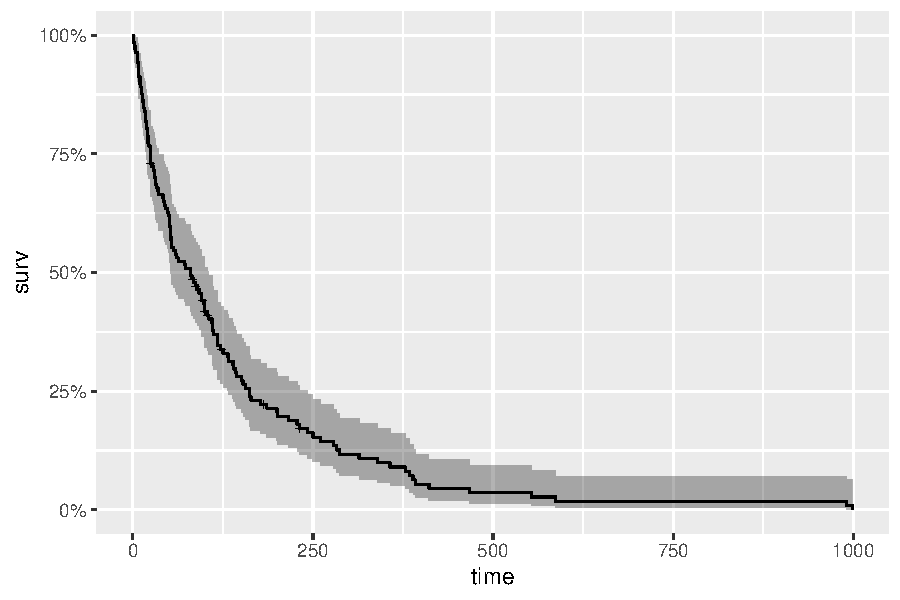
\includegraphics[width=\maxwidth]{figure/figura1-1} 

}

\caption[Função de Sobrevivência]{Função de Sobrevivência}\label{fig:figura1}
\end{figure}


\end{knitrout}

\begin{knitrout}
\definecolor{shadecolor}{rgb}{0.969, 0.969, 0.969}\color{fgcolor}\begin{kframe}
\begin{alltt}
\hlstd{km_trt_fit} \hlkwb{<-} \hlkwd{survfit}\hlstd{(}\hlkwd{Surv}\hlstd{(time, status)} \hlopt{~} \hlstd{trt,} \hlkwc{data}\hlstd{=veteran)}
\hlkwd{autoplot}\hlstd{(km_trt_fit)}
\end{alltt}
\end{kframe}

{\centering 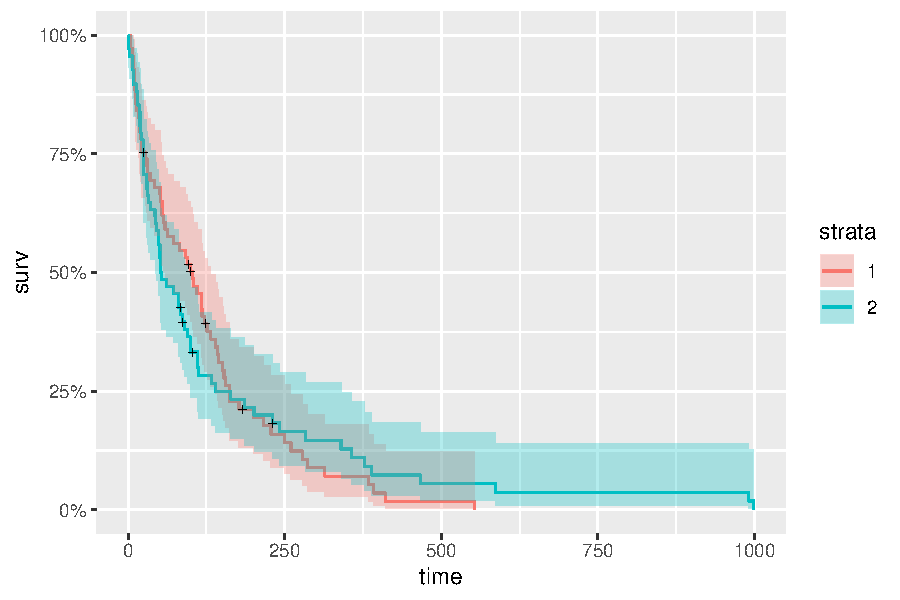
\includegraphics[width=\maxwidth]{figure/script4-1} 

}



\end{knitrout}


\begin{knitrout}
\definecolor{shadecolor}{rgb}{0.969, 0.969, 0.969}\color{fgcolor}\begin{kframe}
\begin{alltt}
\hlstd{vet} \hlkwb{<-} \hlkwd{mutate}\hlstd{(veteran,} \hlkwc{AG} \hlstd{=} \hlkwd{ifelse}\hlstd{((age} \hlopt{<} \hlnum{60}\hlstd{),} \hlstr{"LT60"}\hlstd{,} \hlstr{"OV60"}\hlstd{),}
              \hlkwc{AG} \hlstd{=} \hlkwd{factor}\hlstd{(AG),}
              \hlkwc{trt} \hlstd{=} \hlkwd{factor}\hlstd{(trt,}\hlkwc{labels}\hlstd{=}\hlkwd{c}\hlstd{(}\hlstr{"standard"}\hlstd{,}\hlstr{"test"}\hlstd{)),}
              \hlkwc{prior} \hlstd{=} \hlkwd{factor}\hlstd{(prior,}\hlkwc{labels}\hlstd{=}\hlkwd{c}\hlstd{(}\hlstr{"N0"}\hlstd{,}\hlstr{"Yes"}\hlstd{)))}

\hlstd{km_AG_fit} \hlkwb{<-} \hlkwd{survfit}\hlstd{(}\hlkwd{Surv}\hlstd{(time, status)} \hlopt{~} \hlstd{AG,} \hlkwc{data}\hlstd{=vet)}
\hlkwd{autoplot}\hlstd{(km_AG_fit)}
\end{alltt}
\end{kframe}

{\centering 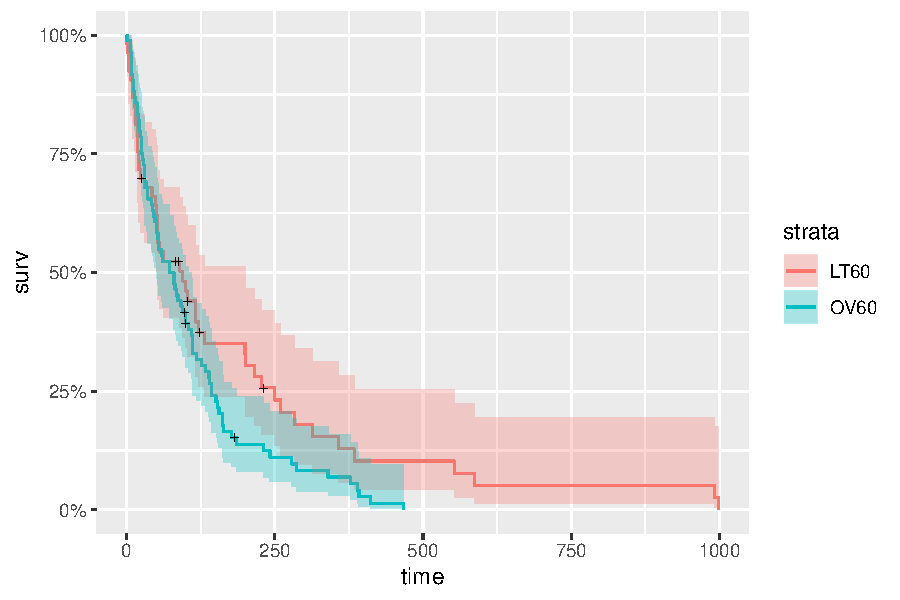
\includegraphics[width=\maxwidth]{figure/script5-1} 

}



\end{knitrout}



      
      
      
      
      \section{Modelo de Riscos Proporcionais de Cox}
      
\begin{knitrout}
\definecolor{shadecolor}{rgb}{0.969, 0.969, 0.969}\color{fgcolor}\begin{kframe}
\begin{alltt}
\hlcom{# Fit Cox Model}
\hlstd{cox} \hlkwb{<-} \hlkwd{coxph}\hlstd{(}\hlkwd{Surv}\hlstd{(time, status)} \hlopt{~} \hlstd{trt} \hlopt{+} \hlstd{celltype} \hlopt{+} \hlstd{karno}                   \hlopt{+} \hlstd{diagtime} \hlopt{+} \hlstd{age} \hlopt{+} \hlstd{prior ,} \hlkwc{data} \hlstd{= vet)}
\hlkwd{summary}\hlstd{(cox)}
\end{alltt}
\begin{verbatim}
## Call:
## coxph(formula = Surv(time, status) ~ trt + celltype + karno + 
##     diagtime + age + prior, data = vet)
## 
##   n= 137, number of events= 128 
## 
##                         coef  exp(coef)   se(coef)      z Pr(>|z|)    
## trttest            2.946e-01  1.343e+00  2.075e-01  1.419  0.15577    
## celltypesmallcell  8.616e-01  2.367e+00  2.753e-01  3.130  0.00175 ** 
## celltypeadeno      1.196e+00  3.307e+00  3.009e-01  3.975 7.05e-05 ***
## celltypelarge      4.013e-01  1.494e+00  2.827e-01  1.420  0.15574    
## karno             -3.282e-02  9.677e-01  5.508e-03 -5.958 2.55e-09 ***
## diagtime           8.132e-05  1.000e+00  9.136e-03  0.009  0.99290    
## age               -8.706e-03  9.913e-01  9.300e-03 -0.936  0.34920    
## priorYes           7.159e-02  1.074e+00  2.323e-01  0.308  0.75794    
## ---
## Signif. codes:  0 '***' 0.001 '**' 0.01 '*' 0.05 '.' 0.1 ' ' 1
## 
##                   exp(coef) exp(-coef) lower .95 upper .95
## trttest              1.3426     0.7448    0.8939    2.0166
## celltypesmallcell    2.3669     0.4225    1.3799    4.0597
## celltypeadeno        3.3071     0.3024    1.8336    5.9647
## celltypelarge        1.4938     0.6695    0.8583    2.5996
## karno                0.9677     1.0334    0.9573    0.9782
## diagtime             1.0001     0.9999    0.9823    1.0182
## age                  0.9913     1.0087    0.9734    1.0096
## priorYes             1.0742     0.9309    0.6813    1.6937
## 
## Concordance= 0.736  (se = 0.021 )
## Likelihood ratio test= 62.1  on 8 df,   p=2e-10
## Wald test            = 62.37  on 8 df,   p=2e-10
## Score (logrank) test = 66.74  on 8 df,   p=2e-11
\end{verbatim}
\begin{alltt}
\hlstd{cox_fit} \hlkwb{<-} \hlkwd{survfit}\hlstd{(cox)}
\hlcom{#plot(cox_fit, main = "cph model", xlab="Days")}
\hlkwd{autoplot}\hlstd{(cox_fit)}
\end{alltt}
\end{kframe}

{\centering 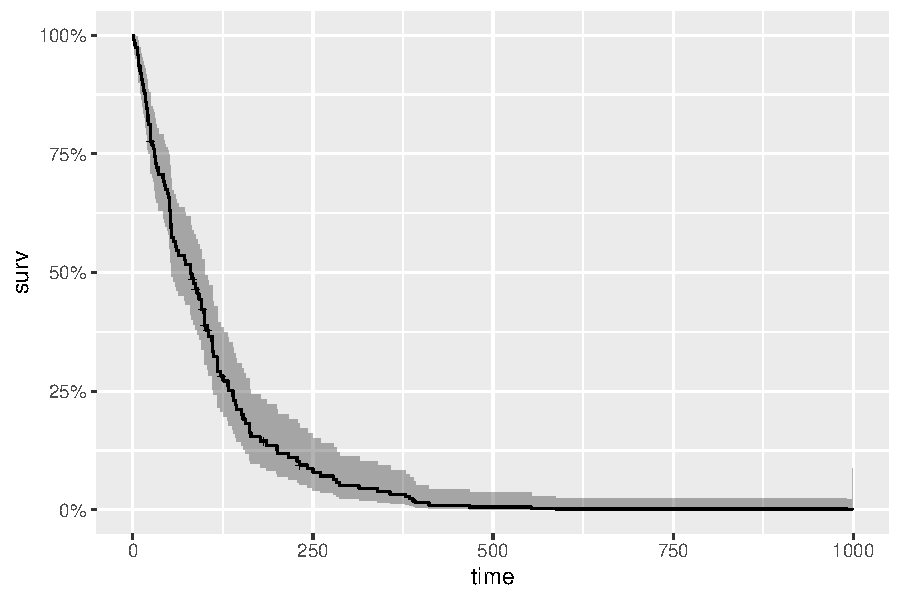
\includegraphics[width=\maxwidth]{figure/script6-1} 

}



\end{knitrout}



\begin{knitrout}
\definecolor{shadecolor}{rgb}{0.969, 0.969, 0.969}\color{fgcolor}\begin{kframe}
\begin{alltt}
\hlstd{aa_fit} \hlkwb{<-}\hlkwd{aareg}\hlstd{(}\hlkwd{Surv}\hlstd{(time, status)} \hlopt{~} \hlstd{trt} \hlopt{+} \hlstd{celltype} \hlopt{+}
                 \hlstd{karno} \hlopt{+} \hlstd{diagtime} \hlopt{+} \hlstd{age} \hlopt{+} \hlstd{prior ,}
                 \hlkwc{data} \hlstd{= vet)}
\hlstd{aa_fit}
\end{alltt}
\begin{verbatim}
## Call:
## aareg(formula = Surv(time, status) ~ trt + celltype + karno + 
##     diagtime + age + prior, data = vet)
## 
##   n= 137 
##     75 out of 97 unique event times used
## 
##                       slope      coef se(coef)      z        p
## Intercept          0.083400  3.81e-02 1.09e-02  3.490 4.79e-04
## trttest            0.006730  2.49e-03 2.58e-03  0.967 3.34e-01
## celltypesmallcell  0.015000  7.30e-03 3.38e-03  2.160 3.09e-02
## celltypeadeno      0.018400  1.03e-02 4.20e-03  2.450 1.42e-02
## celltypelarge     -0.001090 -6.21e-04 2.71e-03 -0.229 8.19e-01
## karno             -0.001180 -4.37e-04 8.77e-05 -4.980 6.28e-07
## diagtime          -0.000243 -4.92e-05 1.64e-04 -0.300 7.65e-01
## age               -0.000246 -6.27e-05 1.28e-04 -0.491 6.23e-01
## priorYes           0.003300  1.54e-03 2.86e-03  0.539 5.90e-01
## 
## Chisq=41.62 on 8 df, p=1.6e-06; test weights=aalen
\end{verbatim}
\begin{alltt}
\hlcom{#summary(aa_fit)  # provides a more complete summary of results}
\hlkwd{autoplot}\hlstd{(aa_fit)}
\end{alltt}
\end{kframe}

{\centering 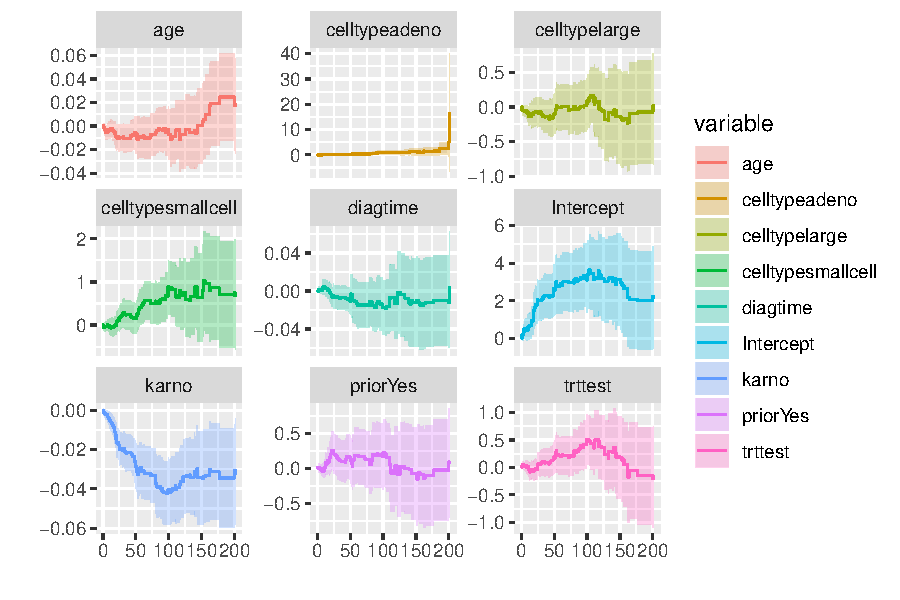
\includegraphics[width=\maxwidth]{figure/script7-1} 

}



\end{knitrout}


      
  \chapter{Resultados e Discusões}

  
  
  
  \chapter{Considerações Finais}
  
  

\bibliography{bibliography}

\end{document}
